\documentclass[11pt]{article}

\usepackage[margin=0.78in]{geometry}
\usepackage{booktabs}
\usepackage{tabularx}
\usepackage{array}
\usepackage{xcolor}
\usepackage{tikz}
\usetikzlibrary{positioning,arrows.meta,calc}
\usepackage{tcolorbox}
\usepackage{enumitem}
\usepackage{lmodern}
\usepackage{microtype}
\usepackage{hyperref}
\usepackage{fancyhdr}
\usepackage{titlesec}
\usepackage{ragged2e}

\hypersetup{colorlinks=true, linkcolor=blue!50!black, urlcolor=blue!50!black}

\definecolor{navy}{RGB}{25,42,70}
\definecolor{blue}{RGB}{44,104,175}
\definecolor{green}{RGB}{70,145,90}
\definecolor{orange}{RGB}{221,137,48}
\definecolor{red}{RGB}{198,76,76}
\definecolor{graytext}{RGB}{78,82,90}
\definecolor{linegray}{RGB}{224,228,235}
\definecolor{lightblue}{RGB}{239,246,255}
\definecolor{lightgreen}{RGB}{240,250,244}
\definecolor{lightorange}{RGB}{255,248,237}
\definecolor{lightred}{RGB}{255,244,244}
\definecolor{panel}{RGB}{247,249,252}

\setlength{\parindent}{0pt}
\setlength{\parskip}{0.45em}
\setlist[itemize]{leftmargin=1.25em,itemsep=0.18em,topsep=0.2em}
\setlist[enumerate]{leftmargin=1.25em,itemsep=0.18em,topsep=0.2em}
\renewcommand{\arraystretch}{1.12}

\titleformat{\section}{\Large\bfseries\color{navy}}{}{0em}{}[\vspace{-0.25em}\color{linegray}\titlerule]
\titleformat{\subsection}{\normalsize\bfseries\color{blue}}{}{0em}{}
\titlespacing*{\section}{0pt}{0.45em}{0.4em}
\titlespacing*{\subsection}{0pt}{0.45em}{0.1em}

\pagestyle{fancy}
\fancyhf{}
\lhead{\small\color{graytext} Cell Placement Optimization}
\rhead{\small\color{graytext} Omar Ramadan}
\cfoot{\small\color{graytext}\thepage}
\renewcommand{\headrulewidth}{0.25pt}

\newtcolorbox{plainbox}[1]{colback=panel,colframe=blue!45!black,title=#1,fonttitle=\bfseries,arc=2mm,boxrule=0.6pt,left=7pt,right=7pt,top=6pt,bottom=6pt}
\newtcolorbox{resultbox}{colback=lightgreen,colframe=green!70!black,arc=2mm,boxrule=0.7pt,left=7pt,right=7pt,top=6pt,bottom=6pt}
\newtcolorbox{warningbox}{colback=lightorange,colframe=orange!80!black,arc=2mm,boxrule=0.7pt,left=7pt,right=7pt,top=6pt,bottom=6pt}
\newtcolorbox{proofbox}{colback=lightblue,colframe=blue!70!black,arc=2mm,boxrule=0.7pt,left=7pt,right=7pt,top=6pt,bottom=6pt}

\tikzset{
    box/.style={draw=blue!60!black, fill=lightblue, rounded corners=2pt, align=center, font=\scriptsize, minimum height=0.72cm, text width=2.25cm},
    good/.style={draw=green!70!black, fill=lightgreen, rounded corners=2pt, align=center, font=\scriptsize, minimum height=0.72cm, text width=2.25cm},
    warn/.style={draw=orange!75!black, fill=lightorange, rounded corners=2pt, align=center, font=\scriptsize, minimum height=0.72cm, text width=2.25cm},
    bad/.style={draw=red!75!black, fill=lightred, rounded corners=2pt, align=center, font=\scriptsize, minimum height=0.72cm, text width=2.25cm},
    arrow/.style={-{Stealth[length=2mm]}, line width=0.8pt, draw=orange!85!black},
    cell/.style={draw=green!70!black, fill=green!18, rounded corners=1pt, line width=0.7pt},
    macro/.style={draw=blue!80!black, fill=blue!16, rounded corners=2pt, line width=0.9pt},
    overlap/.style={draw=red!80!black, fill=red!22, rounded corners=1pt, line width=0.8pt},
    wire/.style={draw=orange!85!black, line width=0.8pt},
    panel/.style={draw=linegray, fill=panel, rounded corners=3pt}
}

\newcommand{\simpleFlow}{%
\begin{center}
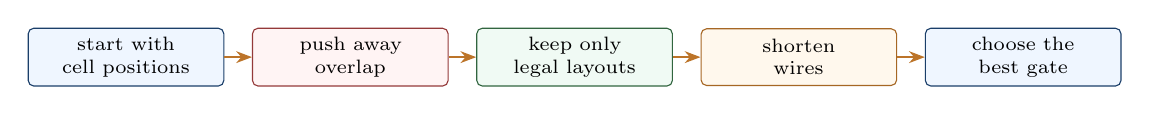
\begin{tikzpicture}[node distance=0.35cm]
\node[box] (start) {start with\\cell positions};
\node[bad, right=of start] (overlap) {push away\\overlap};
\node[good, right=of overlap] (legal) {keep only\\legal layouts};
\node[warn, right=of legal] (wl) {shorten\\wires};
\node[box, right=of wl] (gate) {choose the\\best gate};
\draw[arrow] (start) -- (overlap);
\draw[arrow] (overlap) -- (legal);
\draw[arrow] (legal) -- (wl);
\draw[arrow] (wl) -- (gate);
\end{tikzpicture}
\end{center}}

\newcommand{\overlapDiagram}{%
\begin{center}
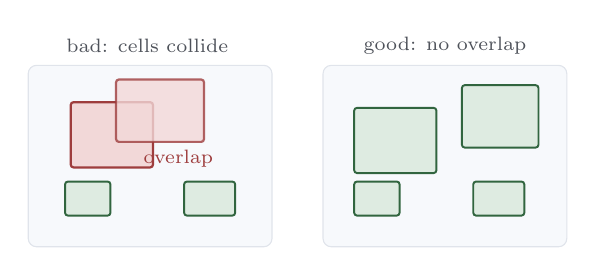
\begin{tikzpicture}[x=0.72cm,y=0.72cm]
\draw[panel] (-0.2,-0.2) rectangle (4.1,3.0);
\node[font=\scriptsize, color=graytext] at (1.9,3.35) {bad: cells collide};
\draw[overlap] (0.55,1.2) rectangle (2.0,2.35);
\draw[overlap, opacity=0.80] (1.35,1.65) rectangle (2.9,2.75);
\draw[cell] (0.45,0.35) rectangle (1.25,0.95);
\draw[cell] (2.55,0.35) rectangle (3.45,0.95);
\node[font=\scriptsize, color=red!80!black] at (2.45,1.35) {overlap};
\draw[panel] (5.0,-0.2) rectangle (9.3,3.0);
\node[font=\scriptsize, color=graytext] at (7.15,3.35) {good: no overlap};
\draw[cell] (5.55,1.1) rectangle (7.0,2.25);
\draw[cell] (7.45,1.55) rectangle (8.8,2.65);
\draw[cell] (5.55,0.35) rectangle (6.35,0.95);
\draw[cell] (7.65,0.35) rectangle (8.55,0.95);
\end{tikzpicture}
\end{center}}

\newcommand{\macroDiagram}{%
\begin{center}
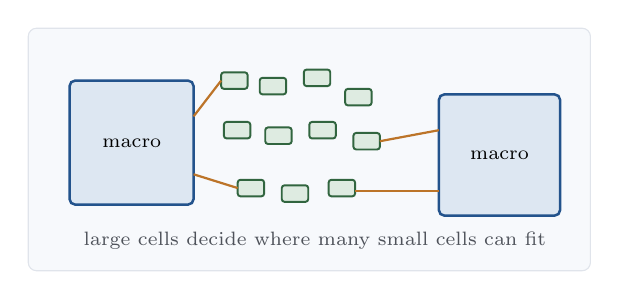
\begin{tikzpicture}[x=0.70cm,y=0.70cm]
\draw[panel] (-0.2,-0.2) rectangle (10.0,4.2);
\draw[macro] (0.55,1.0) rectangle (2.8,3.25);
\node[font=\scriptsize] at (1.68,2.12) {macro};
\draw[macro] (7.25,0.8) rectangle (9.45,3.0);
\node[font=\scriptsize] at (8.35,1.9) {macro};
\foreach \x/\y in {3.3/3.1,4.0/3.0,4.8/3.15,5.55/2.8,3.35/2.2,4.1/2.1,4.9/2.2,5.7/2.0,3.6/1.15,4.4/1.05,5.25/1.15}
    \draw[cell] (\x,\y) rectangle +(0.48,0.30);
\draw[wire] (2.8,2.6) -- (3.3,3.25);
\draw[wire] (2.8,1.55) -- (3.6,1.30);
\draw[wire] (7.25,2.35) -- (6.18,2.15);
\draw[wire] (7.25,1.25) -- (5.72,1.25);
\node[font=\scriptsize, color=graytext] at (5.0,0.35) {large cells decide where many small cells can fit};
\end{tikzpicture}
\end{center}}

\newcommand{\unlockDiagram}{%
\begin{center}
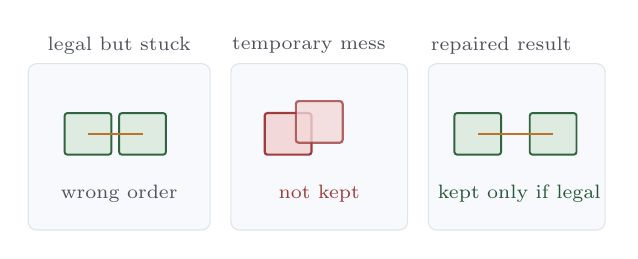
\begin{tikzpicture}[x=0.66cm,y=0.66cm]
\node[font=\scriptsize, color=graytext] at (1.55,3.35) {legal but stuck};
\draw[panel] (-0.2,-0.2) rectangle (3.3,3.0);
\draw[cell] (0.5,1.25) rectangle (1.4,2.05);
\draw[cell] (1.55,1.25) rectangle (2.45,2.05);
\draw[wire] (0.95,1.65) -- (2.0,1.65);
\node[font=\scriptsize, color=graytext] at (1.55,0.50) {wrong order};
\node[font=\scriptsize, color=graytext] at (5.2,3.35) {temporary mess};
\draw[panel] (3.7,-0.2) rectangle (7.1,3.0);
\draw[overlap] (4.35,1.25) rectangle (5.25,2.05);
\draw[overlap, opacity=0.78] (4.95,1.48) rectangle (5.85,2.28);
\node[font=\scriptsize, color=red!80!black] at (5.4,0.50) {not kept};
\node[font=\scriptsize, color=graytext] at (8.9,3.35) {repaired result};
\draw[panel] (7.5,-0.2) rectangle (10.9,3.0);
\draw[cell] (8.0,1.25) rectangle (8.9,2.05);
\draw[cell] (9.45,1.25) rectangle (10.35,2.05);
\draw[wire] (8.45,1.65) -- (9.9,1.65);
\node[font=\scriptsize, color=green!60!black] at (9.25,0.50) {kept only if legal};
\end{tikzpicture}
\end{center}}

\begin{document}

% PAGE 1
\begin{center}
{\Huge\bfseries\color{navy} Cell Placement Optimization}\\[0.25em]
{\Large\color{graytext} A technical summary of the solver and verifier}\\[0.8em]
{\large Omar Ramadan}
\end{center}

\begin{resultbox}
\textbf{Reported local benchmark run.} Running the first ten challenge tests with \texttt{python3 test.py} reached zero average overlap, average wirelength of \textbf{0.250709}, and total runtime of \textbf{858.10 seconds}.
\end{resultbox}

\simpleFlow

\begin{plainbox}{Main idea}
The task is to place rectangles on a chip-like plane. Pins on those rectangles are connected by wires. A good placement has no rectangle collisions and short wires. The solver improved in stages: first remove collisions, then shorten wires, then escape stuck layouts, then choose the best rule for each test case.
\end{plainbox}

\begin{plainbox}{What this report explains}
\begin{itemize}
    \item The optimization goal in everyday language.
    \item The solver tools, with one simple explanation for each.
    \item The gated strategy that chooses different tools for different case shapes.
    \item The proof tools, including the MILP verifier, explained as decision trees and lower bounds.
\end{itemize}
\end{plainbox}

\newpage

% PAGE 2
\section{1. The Problem in Simple Terms}

\begin{plainbox}{Placement}
A placement is a drawing of all cells on a plane. Each cell has a width, height, and center position. Standard cells are small. Macros are large. Pins sit inside cells. Wires connect pins.
\end{plainbox}

\overlapDiagram

\begin{tabularx}{\textwidth}{>{\bfseries\color{navy}}p{0.22\textwidth}X}
Overlap & Two cells occupy the same physical space. This is the first thing the solver must remove. \\
Wirelength & A measure of how long the connected wires are. Shorter is better, but only after overlap is zero. \\
Legal placement & A placement with no overlapping cells. Legal does not mean best; it means allowed. \\
Macro & A large cell. Moving one macro can change the available space for many small cells. \\
Standard cell & A small cell. These are easier to move, assign, and swap. \\
\end{tabularx}

\begin{warningbox}
The two goals fight each other. Wirelength pulls connected cells together. The no-overlap rule pushes cells apart. The solver must shorten wires without breaking legality.
\end{warningbox}

\section{2. What "Optimized" Meant Over Time}

\begin{tabularx}{\textwidth}{>{\bfseries\color{navy}}p{0.25\textwidth}X}
Movable & The cells respond to useful pressure. Overlapping cells can be pushed apart. \\
Legal & The solver finds zero-overlap placements. This is the hard pass/fail rule. \\
Shorter & Once legal, the solver tries to reduce wirelength. \\
Unlocked & The solver temporarily allows a small local mess so cells can escape a stuck order. \\
Gated & The solver chooses the best refinement rule for the shape of the test case. \\
\end{tabularx}

\newpage

% PAGE 3
\section{3. The Solver Pipeline}

The final solver is a portfolio. A portfolio means the solver tries several candidate paths and keeps the best legal result.

\begin{center}
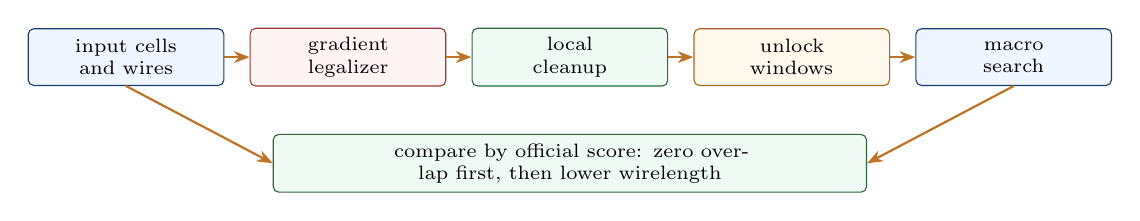
\begin{tikzpicture}[node distance=0.32cm]
\node[box] (input) {input cells\\and wires};
\node[bad, right=of input] (grad) {gradient\\legalizer};
\node[good, right=of grad] (local) {local\\cleanup};
\node[warn, right=of local] (unlock) {unlock\\windows};
\node[box, right=of unlock] (macro) {macro\\search};
\node[good, below=0.6cm of local, text width=7.3cm] (keep) {compare by official score: zero overlap first, then lower wirelength};
\draw[arrow] (input) -- (grad);
\draw[arrow] (grad) -- (local);
\draw[arrow] (local) -- (unlock);
\draw[arrow] (unlock) -- (macro);
\draw[arrow] (input.south) -- (keep.west);
\draw[arrow] (macro.south) -- (keep.east);
\end{tikzpicture}
\end{center}

\begin{tabularx}{\textwidth}{>{\bfseries\color{navy}}p{0.28\textwidth}X}
Gradient legalizer & Moves cell positions step by step. Wires pull connected pins together. Overlap pushes cells apart. \\
Overlap loss & A penalty that grows when rectangles collide. It makes collisions visible to the optimizer. \\
Wirelength loss & A pressure that rewards shorter connected wires. It is used carefully because it can pull cells into overlap. \\
KD-tree pruning & A speed trick for large cases. It checks likely-nearby cells instead of every possible pair. \\
Squeeze portfolio & Gently compresses a legal layout and re-legalizes it. It is kept only if it is still legal and shorter. \\
Final selection & No method is trusted by name. A candidate wins only if it has better official metrics. \\
\end{tabularx}

\begin{plainbox}{The rule that keeps the solver honest}
A zero-overlap candidate beats any overlapping candidate. If both candidates have zero overlap, the one with shorter wirelength wins.
\end{plainbox}

\newpage

% PAGE 4
\section{4. Local Refinement Tools}

Local refinement starts after the solver has a legal placement. The goal is to shorten wires without breaking the no-overlap rule.

\begin{tabularx}{\textwidth}{>{\bfseries\color{navy}}p{0.26\textwidth}X}
Legal projection & Move a cell toward a useful target, but stop at a nearby legal spot if the direct target is blocked. \\
Bandit local search & Try several local move styles and give more attempts to the ones that recently helped. This is not a full learning system; it is a small controller for choosing moves. \\
Same-size assignment & If standard cells have the same size, they can trade legal slots. The solver chooses the slot assignment that shortens wires. \\
Pairwise swaps & Try swapping two cells. Keep the swap only if it stays legal and improves wirelength. \\
Translation-clean scoring & Ignore wires between two pins on the same cell during local move scoring. Moving the cell moves both pins together, so that wire does not change. \\
Partial-move gate & Do not always move a cell all the way to its target. Sometimes a smaller step is safer and scores better. \\
Anchor gate & Keep a stabilizing pull toward a previous good position when that stabilizer improves the measured result. \\
\end{tabularx}

\begin{plainbox}{Why the gates exist}
A cleaner rule did not always win. Translation-clean scoring helped some cases. The anchor gate helped others. The final solver keeps both, then chooses by case shape.
\end{plainbox}

\begin{warningbox}
This is the core engineering lesson: the measured benchmark decided which rule survived. The solver did not keep an idea only because it sounded elegant.
\end{warningbox}

\newpage

% PAGE 5
\section{5. Escaping Stuck Layouts}

A legal placement can still be stuck. No small legal move helps, but a better layout may exist nearby. The solver needs a way to cross that barrier.

\unlockDiagram

\begin{tabularx}{\textwidth}{>{\bfseries\color{navy}}p{0.29\textwidth}X}
Temporary unlock window & Pick a small hot region, allow cells there to overlap during search, then repair the region. The final state must be legal. \\
Relegalization & The repair step. It places the temporarily messy cells back into legal positions. \\
Wirelength-aware repair & During repair, the solver does not simply put cells in the nearest legal spot. It scores candidate spots by whether they shorten important wires. \\
Large-neighborhood search & Move a group of cells together instead of moving one cell at a time. This can change the local ordering of cells. \\
\end{tabularx}

\begin{plainbox}{Simple rule for unlocks}
A messy intermediate state is allowed. A messy final state is never allowed. The result is kept only if overlap is zero and wirelength improves.
\end{plainbox}

\section{6. Macro Search}

\macroDiagram

\begin{tabularx}{\textwidth}{>{\bfseries\color{navy}}p{0.29\textwidth}X}
Macro layout search & Generate different arrangements of the large cells. A different macro arrangement can place the whole design into a different basin. \\
Port-aware relegalization & Place small cells near the macro pins they connect to, while keeping them outside the macro bodies and away from each other. \\
Continuous macro refinement & After a promising macro layout is found, make small coordinate adjustments and rebuild the small-cell placement around it. \\
\end{tabularx}

\newpage

% PAGE 6
\section{7. Ten-Case Gate Profile}

Each case has a different shape. The solver uses the same final rule for every case, but the path to the final candidate can differ.

\begin{center}
\scriptsize
\begin{tabularx}{\textwidth}{>{\bfseries}p{0.06\textwidth}p{0.20\textwidth}p{0.28\textwidth}X}
\toprule
Case & Shape & Main pressure & Gate used \\
\midrule
1 & 22 cells, 2 macros, 20 small cells & Macro placement dominates the small-cell space. & Anchor gate with compact search and macro-shape search. \\
2 & 28 cells, 3 macros, 25 small cells & Small but more macro-constrained than case 1. & Anchor gate with two starting densities and macro-shape search. \\
3 & 32 cells, 2 macros, 30 small cells & Compacting after legality matters. & Anchor gate with squeeze variants. \\
4 & 53 cells, 3 macros, 50 small cells & A spread-out start can avoid bad early packing. & Anchor gate with spread-first and compact retry. \\
5 & 79 cells, 4 macros, 75 small cells & Macro topology still matters, but the small-cell field is denser. & Anchor gate with two macro-density choices. \\
6 & 105 cells, 5 macros, 100 small cells & Same-cell wires can create fake local pressure. & Translation-clean gate with tight start and macro refinement. \\
7 & 155 cells, 5 macros, 150 small cells & Full moves can be too blunt. & Translation-clean gate plus partial-move gate. \\
8 & 157 cells, 7 macros, 150 small cells & Macro-heavy layout where stabilizing pull wins. & Anchor gate plus macro refinement. \\
9 & 208 cells, 8 macros, 200 small cells & Corrected scoring and softer moves both help. & Translation-clean gate plus partial-move gate. \\
10 & 2010 cells, 10 macros, 2000 small cells & Scale matters most. Every pair cannot be checked naively. & Large-design gate with KD-tree checks and squeeze variants. \\
\bottomrule
\end{tabularx}
\end{center}

\begin{resultbox}
\textbf{Final benchmark statement.} The reported local run on the first ten cases reached zero average overlap, an average wirelength of \textbf{0.250709}, and a total runtime of \textbf{858.10 seconds}.
\end{resultbox}

\begin{plainbox}{Why this matters}
The solver became stronger when it stopped forcing one method to explain every test case. The final approach is still systematic: every path must pass the same final legality and wirelength check.
\end{plainbox}

\newpage

% PAGE 7
\section{8. Proofs: What We Can and Cannot Claim}

The solver result is an achieved score. The proof tools ask a different question: how low could any legal placement possibly go?

\begin{proofbox}
\textbf{Lower-bound proof.} A lower bound is a floor. If the proof says the floor is 0.077535, then no placement inside that proof model can go below 0.077535. If our legal score is close to the floor, the proof is strong. If the floor is far below our score, the solver may still be good, but the proof is weak.
\end{proofbox}

\begin{tabularx}{\textwidth}{>{\bfseries\color{navy}}p{0.28\textwidth}X}
Legal upper score & A score we actually achieved with a zero-overlap placement. \\
Lower bound & A certified floor. It says no solution in the proof model can be better than that floor. \\
Gap & The distance between the achieved score and the floor. Smaller gap means stronger proof. \\
Relaxation & A simplified version of the problem. It is easier to prove things about, but it may be too generous. \\
Diagnostic & A helpful numerical check. It improves understanding, but it is not always a formal proof. \\
\end{tabularx}

\begin{warningbox}
The proof folder does not claim global optimality. It documents how close the current evidence gets, which bounds are rigorous, and where the proof is still too loose.
\end{warningbox}

\section{9. The Rigorous Lower-Bound Certificate}

The rigorous certificate breaks the problem into simpler wire questions.

\begin{itemize}
    \item Wires between pins on the same cell are counted exactly.
    \item Wires between different cells are allowed to choose their best pairwise separation.
    \item This is easier than the real placement problem because each pair can choose independently.
\end{itemize}

\begin{center}
\scriptsize
\begin{tabular}{rrrrr}
\toprule
Case & Cells & Total edges & Cell pairs & Lower bound \\
\midrule
1 & 22 & 496 & 78 & 0.169851 \\
2 & 28 & 642 & 153 & 0.120890 \\
3 & 32 & 535 & 176 & 0.108353 \\
4 & 53 & 1091 & 327 & 0.104590 \\
5 & 79 & 1339 & 598 & 0.073179 \\
6 & 105 & 1821 & 883 & 0.059391 \\
7 & 155 & 2247 & 1268 & 0.051953 \\
8 & 157 & 2351 & 1416 & 0.042874 \\
9 & 208 & 2997 & 2003 & 0.036750 \\
10 & 2010 & 20149 & 19394 & 0.007519 \\
\bottomrule
\end{tabular}
\end{center}

The average lower bound from this rigorous run was \textbf{0.077535}. The verified solver average wirelength is \textbf{0.250709}. The earlier bundled diagnostic estimate averaged \textbf{0.154918}, but that number should be treated as diagnostic unless its convex subproblems are independently certified.

\newpage

% PAGE 8
\section{10. LP and MILP Verification}

\begin{proofbox}
\textbf{LP tangent diagnostic.} The LP diagnostic keeps one shared position for every cell. It replaces the curved wire cost with safe straight-line floors. These straight lines sit below the real wire cost, so the model gives a valid lower-bound relaxation. Because it is solved in floating point, the reported number is treated as a residual-audited diagnostic rather than an exact-arithmetic proof.
\end{proofbox}

\begin{proofbox}
\textbf{MILP branch-and-bound verifier.} The verifier turns placement into a yes-or-no search problem. For every selected pair of cells, it asks whether one cell is left, right, above, or below the other. Those choices are discrete, so the solver branches over them like a decision tree. Inside each branch, it computes the best possible wirelength lower bound. If every branch has a lower bound no better than the current legal score, then the current placement is certified optimal inside that bounded proof model.
\end{proofbox}

\begin{tabularx}{\textwidth}{>{\bfseries\color{navy}}p{0.27\textwidth}X}
Coordinate box & A safe search area. The verifier needs this so it does not search infinitely far away. \\
Big-M rule & A switch. When one side choice is active, the other side rules are relaxed. \\
Tangent cut & A safe straight-line floor under the curved wire cost. More tangent cuts make the floor tighter. \\
LP fallback & If the yes-or-no search times out, the solver solves an easier version with relaxed choices. It is safe but weaker. \\
Z3 exact checker & A separate checker that can prove small rationalized models without relying only on floating-point output. \\
\end{tabularx}

\begin{center}
\scriptsize
\begin{tabular}{rrrrr}
\toprule
Case & Different-cell edges used & Planes & LP lower bound & Residual \\
\midrule
1 & 366 & 33 & 0.271042 & 1.07e-14 \\
2 & 506 & 33 & 0.243607 & 7.11e-15 \\
3 & 454 & 33 & 0.227230 & 3.55e-15 \\
4 & 942 & 33 & 0.198941 & 2.49e-14 \\
5 & 1228 & 33 & 0.146962 & 1.78e-14 \\
6 & 1712 & 33 & 0.120244 & 8.08e-14 \\
7 & 2137 & 33 & 0.124031 & 3.55e-14 \\
8 & 2269 & 33 & 0.102329 & 3.87e-14 \\
9 & 2928 & 33 & 0.086376 & 4.62e-14 \\
10 & 3000 subset & 33 & 0.010510 & 9.95e-14 \\
\bottomrule
\end{tabular}
\end{center}

The average LP diagnostic lower bound was \textbf{0.153127}. The average capped MILP lower bound from the latest rerun was \textbf{0.153193}.

\newpage

% PAGE 9
\section{11. MILP Results and Exact-Check Boundary}

The all-case capped MILP run used \textbf{600} selected cell pairs, \textbf{3000} selected different-cell wires, a position bound of \textbf{500}, and a \textbf{ten-second} MILP budget per case.

\begin{center}
\scriptsize
\begin{tabular}{rrrrr}
\toprule
Case & Different-cell edges used & Pairs used & MILP lower bound & Scope \\
\midrule
1 & 366 of 366 & 231 of 231 & 0.271042 & full, LP fallback \\
2 & 506 of 506 & 378 of 378 & 0.243607 & full, LP fallback \\
3 & 454 of 454 & 496 of 496 & 0.227230 & full, LP fallback \\
4 & 942 of 942 & 600 of 1378 & 0.198941 & capped \\
5 & 1228 of 1228 & 600 of 3081 & 0.146962 & capped \\
6 & 1712 of 1712 & 600 of 5460 & 0.120244 & capped \\
7 & 2137 of 2137 & 600 of 11935 & 0.124031 & capped \\
8 & 2269 of 2269 & 600 of 12246 & 0.102328 & capped \\
9 & 2928 of 2928 & 600 of 21528 & 0.086376 & capped \\
10 & 3000 of 20095 & 600 of 2019045 & 0.011165 & capped \\
\bottomrule
\end{tabular}
\end{center}

\begin{plainbox}{Case-one proof details}
\begin{itemize}
    \item A tight working-box run used a position bound of \textbf{500}. It included every pair, every different-cell wire, and extra tangent points. It produced a lower bound of \textbf{0.333241} after \textbf{6880} branch-and-bound nodes. This is the strongest numeric lower bound, but the coordinate box is not certified from the incumbent.
    \item A coordinate-certified run used the incumbent upper bound to derive a safe position bound of about \textbf{12600}. It included every pair and every different-cell wire, used edge-specific side tangent cuts, and produced a lower bound of \textbf{0.302605}. This is weaker, but the coordinate-box assumption is fixed.
\end{itemize}
\end{plainbox}

\begin{proofbox}
\textbf{Exact checker.} For a capped case-one model with \textbf{144} variables, \textbf{80} binary variables, and \textbf{440} linear constraints, Z3 proved that no modeled placement exists below \textbf{0.05}. This does not close the full proof, but it shows the workflow can produce independently checkable claims on small models.
\end{proofbox}

\newpage

% PAGE 10
\section{12. Global Optimality Attempt and Lessons}

To prove global optimality, the verifier must keep one shared position for every cell and prove that every possible non-overlap ordering is no better than the current legal solution.

\begin{proofbox}
\textbf{Global proof attempt.} The branch-and-bound verifier builds a tree. Each branch chooses one ordering rule for one pair of cells: left, right, below, or above. If a branch cannot possibly beat the current legal score, the verifier cuts it off. If all branches are cut off, the current solution is proven optimal inside that proof model.
\end{proofbox}

The verifier proves a tiny two-cell demo, which confirms the proof architecture works on a case small enough to close. It does not yet prove benchmark case one. A bounded case-one run with \textbf{200} branch nodes raised the rigorous lower bound to \textbf{0.217704465}. The current legal upper bound for that run was \textbf{0.333636141}, leaving an open gap of \textbf{0.115931676}.

\begin{tabularx}{\textwidth}{>{\bfseries\color{navy}}p{0.31\textwidth}X}
What is proven & The edge-independent certificate is a valid floor. Same-cell wires are handled correctly. Small capped MILP claims can be checked independently. \\
What is not proven & The solver is not proven globally optimal on the benchmark. The lower bounds remain too loose for a full near-optimality claim. \\
Why the solver is still strong & It achieves zero overlap and uses measured gates to reduce wirelength across different case shapes. \\
Next proof improvement & Build tighter certified branch lower bounds or run stronger exact solvers on small cases. \\
Next solver improvement & Keep the gated strategy, but focus on large-case detailed placement and cleaner local scoring. \\
\end{tabularx}

\begin{resultbox}
\textbf{Final position.} The submitted placer is a strong heuristic solver. The verification work does not claim global optimality. It shows which lower bounds are rigorous, which checks are diagnostic, and what remains open before a full optimality proof is possible.
\end{resultbox}

\begin{warningbox}
\textbf{Closing Thoughts.} Optimization means the next useful improvement under the current constraint: first movement, then legality, then shorter wires, then escape from stuck layouts, and finally the right gate for each case. The proof work is not the submission's scoring claim. It is included to show that I investigated what can be certified, what is only diagnostic, and where exact optimality becomes computationally difficult.
\end{warningbox}

\end{document}
